% !TeX spellcheck = en_GB
\def\ChapterTitle{Assessment of TMF Performance in Marine Environments}

\chapter{\ChapterTitle}
\label{Chapter\thechapter}
\lhead{Chapter \thechapter. \emph{\nameref{Chapter\thechapter}}} % Write in your own chapter title to set the page header


\section{Introduction}

In this chapter, the need for multi-metric trust assessment in \gls{uan} is demonstrated as an example of a harsh network environment.

In underwater environments, communications is both sparse and noisy.
Therefore the observations about the communications processes that are used to generate trust metrics, occur much less frequently, with much greater error (noise) and delay than is experienced in terrestrial RF \glspl{manet}.

In addition to the communications challenges, other considerations such as command and control isolation, as well as power and locomotive limitations, drive towards the use of teams of smaller and cheaper \glspl{auv}.
As such, the use of trust methods developed in the terrestrial \gls{manet} space must be re-appraised for application within the underwater context \cite{Pavan2015}.
Many \glspl{uan} use \gls{manet} architectures, however the marine environment presents new challenges for trust management frameworks that have been developed for use in conventional (i.e. Terrestrial RF) \glspl{manet}.
Previous research has established the advantages of implementing TMFs in 802.11 based \glspl{manet}, particularly in terms of preventing selfish operation in collaborative systems \cite{Li2007}, and maintaining throughput in the presence of malicious actors \cite{Buchegger2002}

To date this work has been limited to terrestrial, RF based networks. 

The operation of a selection of traditional \gls{manet} \glspl{tmf} in this environment is investigated.
These challenges are characterised and results are presented that demonstrate a multi-metric approach to Trust greatly enhances the effectiveness of TMFs in these environments.

In Section \ref{sec:initialsystemcharacterization} an experimental configuration for the marine space is established, and the scenarios and results presented in \cite{Guo11} are reviewed for comparison.
In Section \ref{sec:trustresultsanddiscussion} findings in trust establishment and malicious behaviour detection are presented and comparing with other current \glspl{tmf} (Hermes and \gls{otmf}) and the use of this multi-parameter approach to detecting malicious and selfish behaviour in autonomous marine networks is analysed.

The contributions of this chapter are a study on the comparative operation and performance of \glspl{tmf} in marine acoustic networks, and a review of metric suitability for \glspl{tmf} in marine environments, informing future metric selection for experimenters and theorists.
It is shown that single metric trust systems are not directly suitable for the marine context in terms of the different threat and cost scenario in that environment.
Finally, a methodology to assess the usefulness of metrics in discriminating against misbehaviours in such constrained, delay-tolerant networks is demonstrated.

Key parts of this chapter were presented at TrustCom-BigDataSE-ISPA 2015 as ``Single and Multi-Metric Trust Management Frameworks for use in Underwater Autonomous Networks.''\cite{Bolster2015}

These single metric \glspl{tmf} provide malicious actors with a significant advantage if their activity does not impact that metric.
In the case where the attacker can subvert the \gls{tmf}, the metric under assessment by that \gls{tmf} does not cover the threat mounted by the attacker.
This causes a significant negative effect on the efficiency of the network, as the TMF is assumed to have reduced the possible set of attacks when it has actually made it more advantageous to attack a different part of the networks operation.
An example of such a situation would be in a \gls{tmf} focused on \gls{plr} where an attacker selectively delays packets going through it, reducing overall throughput but not dropping any packets.
Such behaviour would not be detected by the \gls{tmf}.

For the purposes of this work, from those \glspl{tmf} discussed in~\autoref{sec:c2_tmfs}, select Hermes trust establishment, \gls{otmf} and \gls{mtfm} are selected as indicative single and multi metrics frameworks for comparison, as Hermes captures the core operation of a pure single metric assessment methodology and \gls{otmf} provides a comparison that combines assessments from across nodes to develop trust opinions.

From the discussion on the nature of the communications environment in~\autoref{sec:trust_in_marine}, it's clear that before assessing communications metrics a simulated underwater environment, appropriate scaling factors must be found that are realistic from an application perspective but are also comperable in some form to the \gls{manet} case.

\section{Modelling of \gls{uan} network)\label{sec:initialsystemcharacterization}}


\subsection{Mobility, Topology, and Communications}

Four mobility patterns are investigated:
\begin{enumerate}
	\item All Nodes Static
	\item Malicious node mobile
	\item Malicious node mobile, all other nodes static
	\item All nodes mobile
\end{enumerate}

For this case, the mobility model used is a random walk on the nodes modeled kinematic response, i.e. the node periodically picks a spherically normalised random direction in the XY plane

The reason for this is that in other mobility combinations, the node targeted for misbehaviour ($n_1$) will already be behaving differently compared to the rest of the network regardless of the misbehaviour.
\todo{expand this section to include discussion and results of single mobility models}

The six nodes are initially arranged as per Fig.~\ref{fig:s1_layout} with each node on average 100m from each other as per \cite{Guo11}.
The use of six nodes and the particular layout enables the investigation of the three trust relationships based on minimum path topologies, such that the node generating the trust assessments, $n_0$ has Direct, Recommendation, and Indirect trust assessments of $n_1$ available to it from itself, $[n_2,n_3]$, and $[n_4,n_5]$ respectively. 
(See Section~\ref{sec:trust_topologies})

Collaborations with NATO \gls{cmre} in La Spezia, and \glspl{dstl} Naval Systems Group inform that this is a practical team-size for environmental and defence applications.

%
\begin{figure}[h]
	\centering
	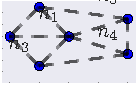
\includegraphics[width=.45\textwidth]{s1_layout}
	\caption{Initial layout with nodes spaced an average of 100m apart}
	\label{fig:s1_layout}
\end{figure}
%

\subsection{Simulation Background}

Simulations were conducted using a Python based simulation framework, SimPy \cite{Mueller2003SimPy}, with a network stack built upon AUVNetSim \cite{Miquel2008}, with transmission parameters (Table \ref{tab:sysconstraints}) taken from and validated against \cite{Stojanovic2007}, \cite{Stefanov2011} and \cite{Sehgal2010}\todo{it would be worth while going through this verification explicitly as an appendix}

Given the differences in delay and propagation between RF and marine networks, it would not be expected that the same application rates (e.g. packet emission rates or throughput) and node separations are equally stable in this environment.
Therefore, a zone of performance is characterised within which the network has stable operation.
%
\begin{table}[h]
	\caption{Comparison of system model constraints as applied between Terrestrial and Marine communications} \label{tab:sysconstraints}
	\begin{center}
		\setlength{\tabcolsep}{8pt}
		\begin{tabular}{lccc}
			\toprule
			Parameter & Unit & Terrestrial & Marine \\
			\midrule
			Simulated Duration & $s$ & 300 & 18000\\
			Trust Sampling Period & $s$ & 1 & 600 \\
			Simulated Area & $km^2$ & 0.7 & 0.7-4 \\
			Transmission Range & $km$ & 0.25 & 1.5 \\
			Physical Layer & & RF(802.11) & Acoustic\\
			Propagation Speed& $m/s$ & $3\times10^8$ & 1490\\
			Center Frequency& $Hz$ & $2.6\times10^9$ & $2 \times 10^4$ \\
			Bandwidth& $Hz$ & $22\times10^6$ & $1\times10^4$\\
			MAC Type & & CSMA/DCF & CSMA/CA\\
			Routing Protocol & & DSDV & FBR \\
			Max Speed & $ms^{-1}$ & 5 & 1.5 \\
			Max Data Rate & $bps$ & $5\times10^6$ & $\approx 240$ \\
			Packet Size & bits & 4096 &  9600 \\
			Single Transmission Duration & $s$ & 10 & 32 \\
			Single Transmission Size & bits & $10^7$ & $9600$ \\
			\bottomrule
		\end{tabular}
		\setlength{\tabcolsep}{6pt}
	\end{center}
\end{table}
%


\subsection{Scaling Considerations between Terrestrial and Underwater Environments}

We establish an appropriate safe operating zone for marine communications by looking at the communications rate and physical distribution factors across the two selected mobility scenarios.
From Table~\ref{tab:sysconstraints}, the operating transmission range of this model of acoustic communications is $\approx 6$ times further than that of 802.11, indicating that a suitable operating environment will have an area $\approx \sqrt{6}$ times the area of the 802.11 case.
However, it was recognised in Section~\ref{sec:marineacousticnetworks} that underwater, the relationship between attenuation and distance is exponential, so this would represent an upper bound of performance, where nodes are approximately $400m$ apart. 

Exploratory simulations were run to further constrain this bound.
As the separation is increased, the emission rate at which the network becomes saturated decreases, reducing overall throughput. 
This throughput degradation is tightly coupled with the mobility, as increasing mobility leads to increasing delays as routes are constantly broken, re-advertised and re-established. 
For instance, where all nodes are static, significant drops in saturation rates are not seen until node separation approaches 800m, nearly double the initial estimate. 
When all nodes are randomly walking the saturation point collapses from $0.025pps$ at $300m$ to $0.015pps$ at $400m$.
Our results indicate that the best area to continue operating in for a range of node separations is at $0.015pps$, and that a reasonable position scaling is from $100m$ to $300m$, beyond which communication becomes increasingly unstable, especially in terms of end-to-end delay.
These results are similar to work performed in \cite{Miquel2008}, and are expected in such a sparse, noisy, and contentious environment. 



\section{Establishing Scale Factors in Communications Rate}

In this section the simulated communications environment is characterised to establish an optimal packet emission rate for comparison against \cite{Guo11}.

In order to establish the point at which the network becomes saturated due, a range of packet emission rates were explored between 0.01 packets per second (pps), equivalent to 96 bps, up to 0.07 pps (672 bps)

From Figs.~\ref{fig:throughput_performance_static} and~\ref{fig:prod_breakdown_static}, it is clear that the threshold curve, expressed as the \emph{Successfully Received Packets} line, exhibits a saturation point between 0.025 and 0.03 pps.
Particularly in Fig.~\ref{fig:prod_breakdown_static}, the precipitous drop in packet delivery probability beyond 0.025 pps, indicating that this is a strong candidate value for an upper-limit to the safe operating zone in terms of packet emission in the small static case.

\begin{figure}[H]
	\centering
	%\missingfigure{throughput_performance_static}
	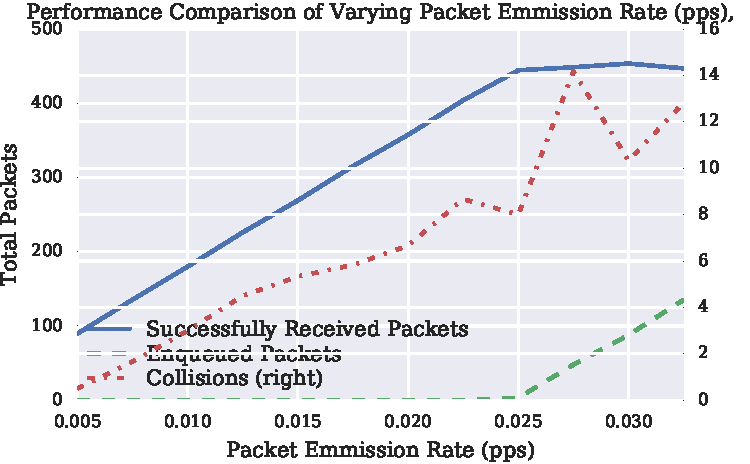
\includegraphics[width=0.8\textwidth]{throughput_performance_static}
	\caption{Varying packet emission rate demonstrates maximal throughput at 0.025 packets per second, equivalent to $\approx$240 bps}
	\label{fig:throughput_performance_static}
\end{figure}


\begin{figure}[H]
	\centering
	%\missingfigure{prod_breakdown_static}
	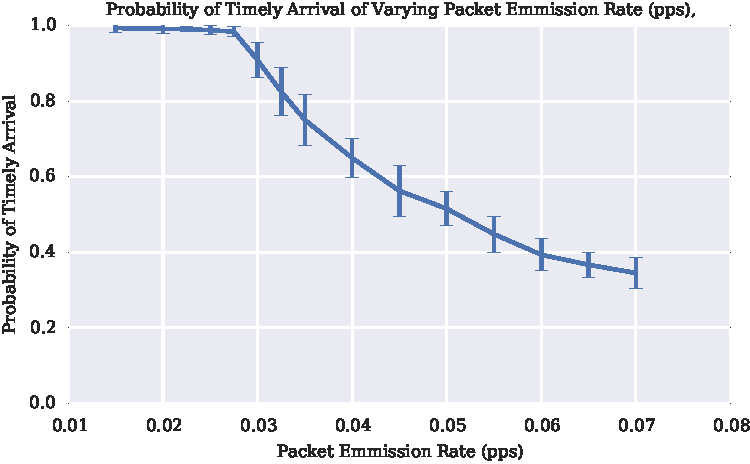
\includegraphics[width=0.8\textwidth]{prod_breakdown_static}
	\caption{Varying packet emission rate demonstrates a saturation point at 0.025 packets per second}
	\label{fig:prod_breakdown_static}
\end{figure}



\subsection{Establishing Scale Factors in Physical Distribution}

In this section the effect of node-separation scaling on communications operation is characterised for comparison against \cite{Guo11}. This is particularly important considering the significant scale factor differences between not only the speed of propagation in the medium, but simply the range of operation. 
From Table~\ref{tab:sysconstraints}, the operating transmission range of acoustic is $\approx 6$ times further than 802.11, indicating that a suitable operating environment will have an area $\approx \sqrt{6}$ times the area of the 802.11 case. Therefore, a reasonable experimental range would have an upper bound of performance around this scaling factor, where nodes are approximately 400$m$ apart. 

A reasonable range around this is to scale from 100$m$ apart on average to 800$m$.

Varying average node separation shows that while direct throughput isn't significantly affected until, collision rates are Fig.~\ref{fig:throughput_performance_range}.
This collision rate is well within the tolerances of the MAC layer, as shown in Fig.~\ref{fig:prod_breakdown_range}, where even with a rising collision rate, packets are being reliably received.

\begin{figure}[H]
	\centering
	%\missingfigure[width=0.6\textwidth]{throughput_performance_range}
	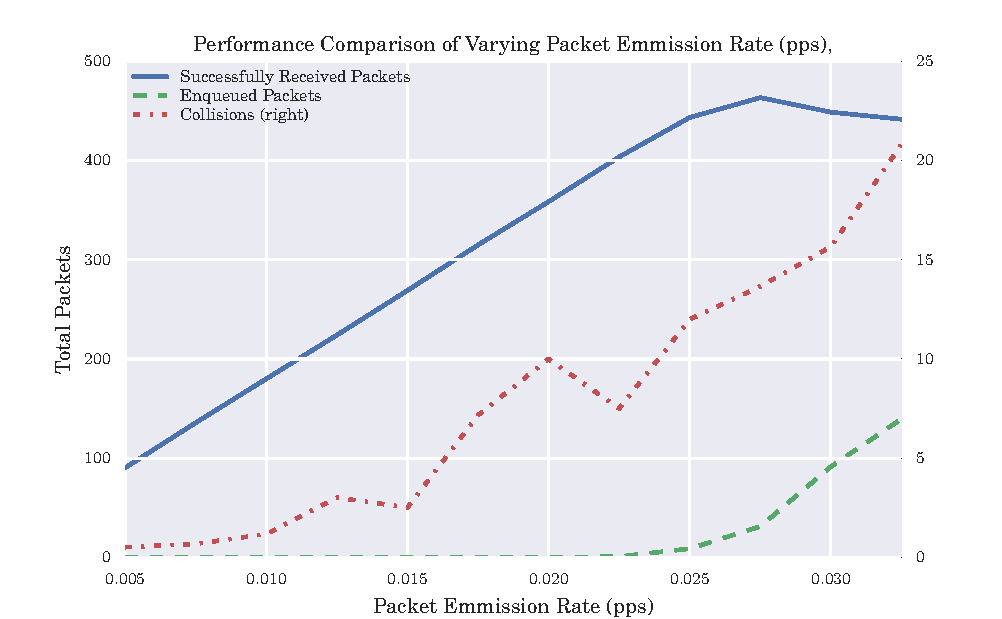
\includegraphics[width=0.8\textwidth]{throughput_performance_bella_all_mobile}
	\caption{Medium Acquisition Collisions, Throughput, and Enqueued packets against varying application packet emission rates for full mobility model}
	\label{fig:throughput_performance_range}
\end{figure}

\begin{figure}[H]
	\centering
	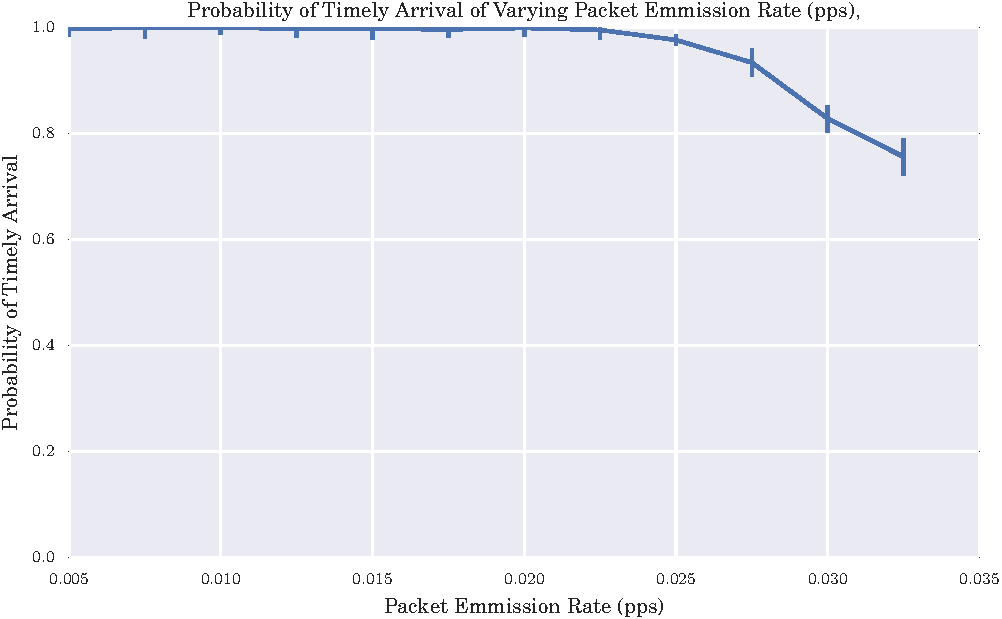
\includegraphics[width=0.8\textwidth]{prod_breakdown_bella_all_mobile}
	\caption{Probability of Timely Reception Varying Node Separation for full mobility model}
	\label{fig:prod_breakdown_range}
\end{figure}

However, when end-to-end delay is investigated, it's clear from Fig.~\ref{fig:delay_range} that the network is becoming severely impaired approaching the 600$m$ mark, with delays rising to more than 25 minutes above 700$m$.
This is also demonstrated by the increasing RTS/Data ratio shown in Fig.~\ref{fig:rts_range}.

According to Xu, the RTS/CTS handshake cannot function well as interference protection at node separations beyond 0.56 times the transmission range \cite{Xu2002}.
This is also demonstrated in~\autoref{fig:rts_range}, where as node separation increases towards $1500m \times 0.56 = 840m$, handshake overheads begin to dominate channel access.\todo{redo these graphs with wider separations ~ 1000m}
This is due to reduced channel availability due to collisions, which are then due to a much longer potential contention period between nodes. 

\begin{figure}[H]
	\centering
	%\missingfigure{delay range}
	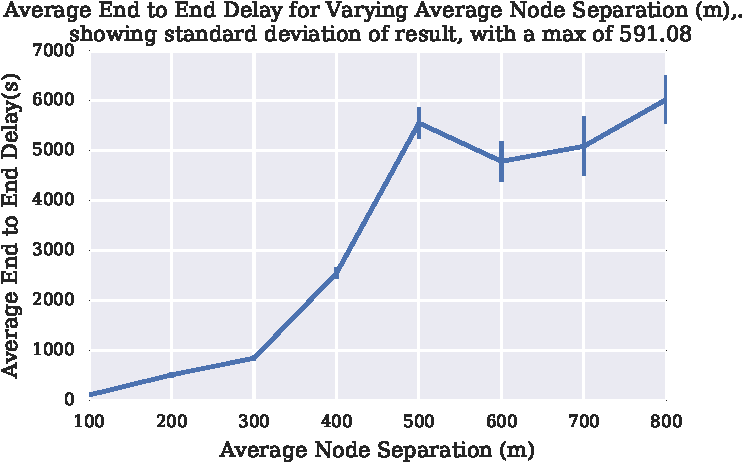
\includegraphics[width=0.8\textwidth]{delay_range}
	\caption{End to End Delay under varying node-separations}
	\label{fig:delay_range}
\end{figure}

\begin{figure}[H]
	\centering
	%\missingfigure{rts range}
  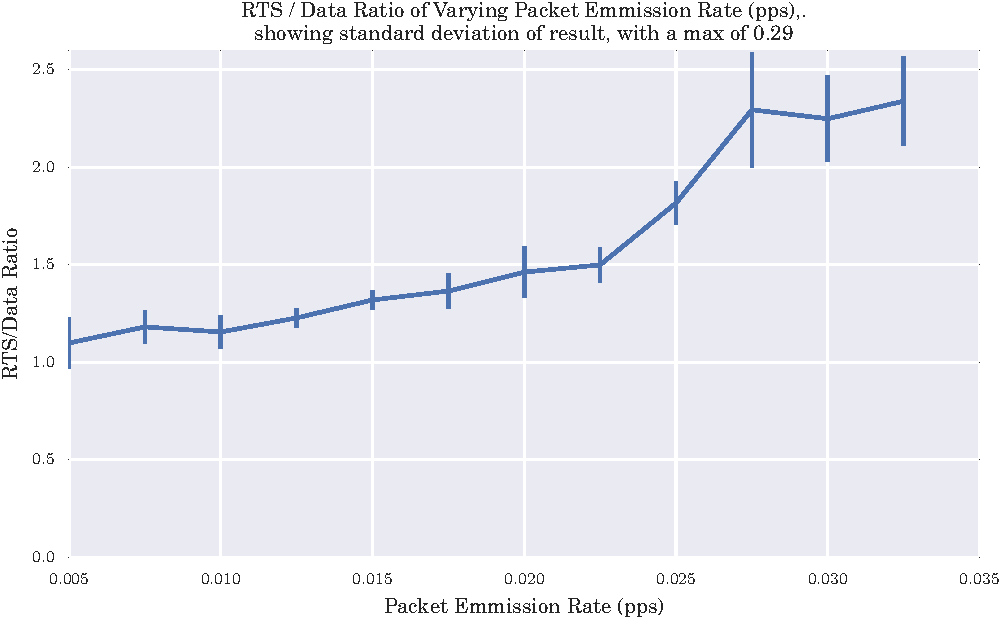
\includegraphics[width=0.8\textwidth]{rts_ratio_bella_static}
	\caption{RTS/Data ratio for varying node-separations}
	\label{fig:rts_range}
\end{figure}


\begin{table}[H]
	\caption{Tabular view of data from Figs~\ref{fig:prod_breakdown_range},~\ref{fig:delay_range}, and~\ref{fig:rts_range}} \label{tab:rangedelay}
	\begin{center}
		\hyphenpenalty 100000
		\begin{tabular}{
				*{2}{@{\hspace{1em}}r@{\hspace{1em}}}
				*{3}{@{\hspace{1em}}p{0.1\textwidth} @{\hspace{1em}}}
      }
			\toprule
			Separation(m) &  Delay(s) &  Probability of Arrival &  RTS/Data Ratio &  Ideal Delivery Time(s) \\
			\midrule
			100 &     60.32 &                    0.99 &            1.80 &                    1.03 \\
			200 &    419.95 &                    0.97 &            2.02 &                    1.10 \\
			300 &   1205.66 &                    0.89 &            2.41 &                    1.17 \\
			400 &   1288.20 &                    0.91 &            2.26 &                    1.25 \\
			500 &   1868.20 &                    0.87 &            2.41 &                    1.32 \\
			600 &   2191.07 &                    0.85 &            2.42 &                    1.39 \\
			\bottomrule
		\end{tabular}
	\end{center}
\end{table}


%%%%%%%%%%%%%%%%%%%%%%%%%%%%%%%%%%%%%%%%%%%%%%%%%%%%%%%%%%%%%%%%%%%%%%%%%%%%%%%
